

\section{Perspectivas de mejora}

Hemos visto que con los detectores de silicio somos capaces de reconstruir las energías de excitación. Sin embargo, con estos no somos capaces de recuperar la cinemática de baja energía. Es aquí donde radica una de las ventajas de la TPC, que nos permite recuperar estadística a partir de un \textit{trigger} interno llamado \textit{L1}, basado en la multiplicidad de los pads de lectura; esto es, en el número de electrones que llega a cada uno de los pads. Este \textit{trigger} se activará cuando el número de \textit{pads} activados sea mayor a un límite impuesto por el usuario.

%non podes ser tan dramático e botar abaixo todo o que fixeches antes. si que se poden sacar cousas, xa che comentei que os fits da anterior sección son posibles e aínda non son tan malos. Tes que motivar isto de forma máis construtiva, para explotar todo o potencial do detector e recuperar os eventos de baixa enerxía do tritio, que se corresponden coa sección eficaz maior

Para que sean medidos satisfactoriamente por este \textit{trigger} \textit{L1} necesitamos que los tritios se frenen en algún punto superior al plano XY de la cámara de deriva, ya que es en esta región de la TPC donde se encuentran los \textit{pads} que mediran los electrones. Sin embargo, no todas las partículas que  se frenen nos servirán para poder reconstruir la cinemática. Si existe ruido en el detector (ruido electrónico, medidas espurias...) estaríamos disparando medidas continuamente en ruido. Además los \textit{pads} tinene una resolución por su tamaño de 2 mm. Estos factores no permiten obtener conclusiones con aquellas partículas que tengan un rango en el gas menor que 20 mm, límite estimado para que las trazas de partículas de interés no tengan ruido.  En la \cref{Fig:06-RangeTheta} podemos ver precisamente el rango de todas las partículas que se frenan respecto el ángulo, y el límite impuesto de $L_{xy}>20$ mm.  

\begin{figure}[H] \centering
    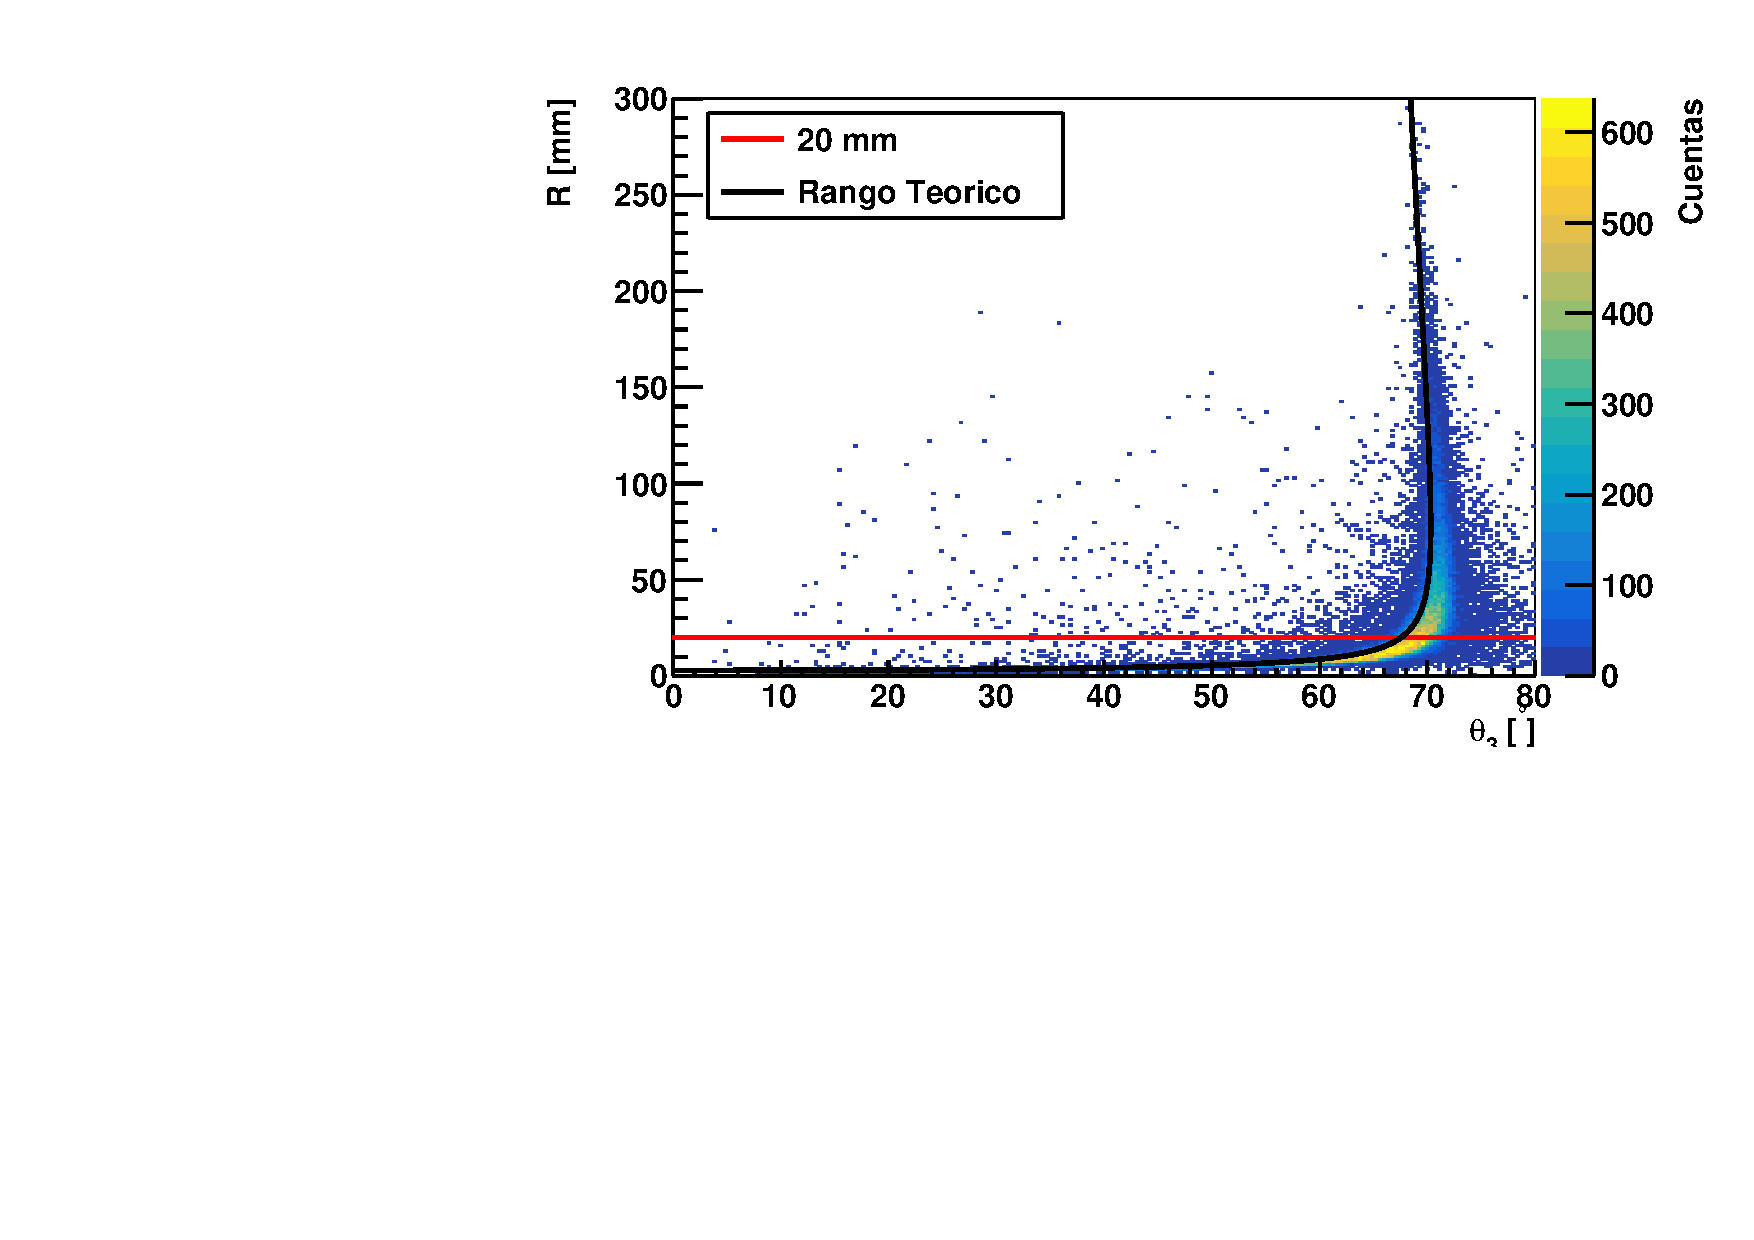
\includegraphics[width=0.73\linewidth]{Imagenes/Trigger/RangeTheta_Ex0.00_incIdx0.pdf}
    \caption{Rango vs $\theta$ de los eventos con $E_x=0.0$ MeV y el rango teórico.}
    \label{Fig:06-RangeTheta}
\end{figure}

Con el siguiente porcentaje de eventos recuperables dentro de todos los que se paran (cociente entre aquellos eventos con rango mayor de 2 cm y todos los que se frenan), tal que: 


\begin{table}[H] \centering
    \begin{tabular}{llll} \hline
\toprule 
$E_{x}=0.0$ MeV & $E_{x}=0.20$ MeV \\ 
 \midrule 
 51.2438\% & 75.0016\% &\\ 
\bottomrule 
\end{tabular}
  
    \caption{porcentaje de eventos recuperables.}
\end{table}

\vspace*{-0.4cm}

Esto nos indica que podremos recuperar una pequeña zona de baja energía que por las características de la sección eficaz y la cinemática se corresponderán a un gran porcentaje sobre los eventos globales. En la \cref{Fig:06-kin-L1} podemos observar la cinemática de los eventos recuperables gracias al Trigger, que como se ve incluye un amplio rango en $\theta$ y cinemática de baja energía.  

\begin{figure}[H] \centering

    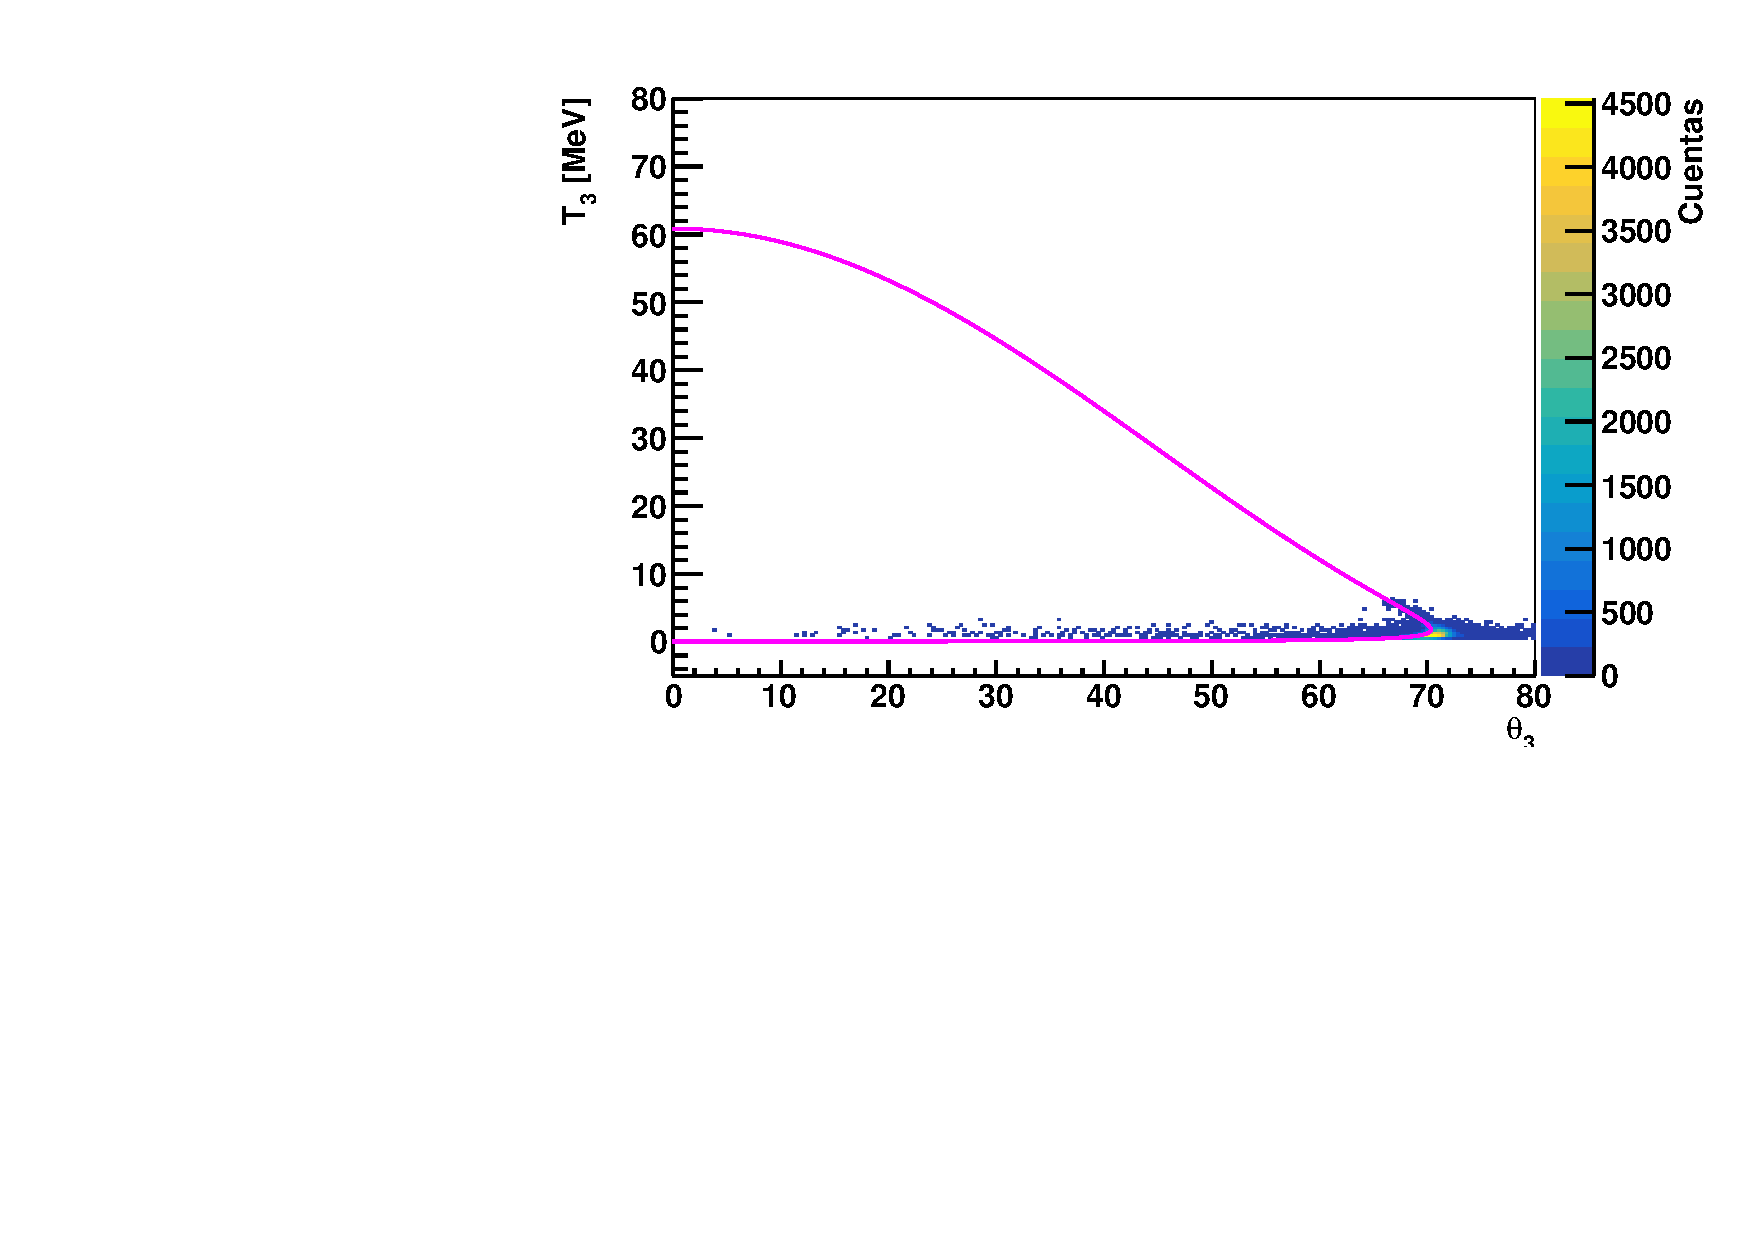
\includegraphics[width=0.73\linewidth]{Imagenes/Trigger/EkinMeasuredL1_Ex0.00_incIdx0.pdf}
    \caption{Cinemática de los eventos que se frenan en la cámara de deriva y que son medidos (con rango $L\geq 20$ mm) con todas las fuentes de incertidumbre y $E_x=0$ MeV.}
    \label{Fig:06-kin-L1}
\end{figure}
